\section{Setting up secure connections}

There is a right (secure) way to configure your connection to your
provider's mail servers and a wrong (insecure) way. The most fundamental
aspect of e-mail security is the type of connection that you make to
your e-mail provider's mail server.

Whenever possible, you should connect using the \textbf{SSL} (Secure
Socket Layer) and \textbf{TLS} (Transport Layer Security) protocols.
(\textbf{STARTTLS}, which is another option available when configuring
an account, is a variation of SSL / TLS.) These protocols prevent your
own system (beyond Thunderbird) and any points between your system and
the mail server from intercepting and obtaining your password. SSL / TLS
also prevent eavesdroppers from reading the content of your messages.

These protocols, however, only secure the connection between your
computer and the mail server. They do not secure the information channel
all the way to the message recipient. Once the mail servers forward the
message for delivery, the message may be intercepted and read by points
in between the mail server and the recipient.

This is where \textbf{PGP} (Pretty Good Privacy) comes in, which is
described in the next chapter.

The first step in establishing e-mail security is a secure connection
between your system and the mail servers. This chapter describes how to
set up your e-mail account the right way.

\subsection{Configuration requirements}

When you configure an account, Thunderbird attempts to determine (from
the email account and the account details that you provide) the
connection parameters to your email provider. While Thunderbird knows
the connection parameters for many email providers, it does not know
them all. If the parameters are not known to Thunderbird, you will need
to provide the following information to configure your account:

\begin{itemize}
\item
  \textbf{Your username}
\item
  \textbf{Your password}
\item
  \textbf{Incoming server:} name (such as \verb!imap.example.com!),
  protocol (POP or IMAP), port (by default, 110), and security protocol
\item
  \textbf{Outgoing server:} name (such as \verb!smtp.example.com!), port
  (by default, 25), and security protocol
\end{itemize}
You should have received this information from your hosting provider.
Alternatively, you can usually find this information on the support
pages on the website of your hosting provider. In our example we will be
using the Gmail server configuration. You can use Thunderbird with your
Gmail account. To do so, you must change a configuration setting in your
account. If you are not using a Gmail account, skip the next section.

\subsection{Preparing a Gmail account for use with Thunderbird}

Log in to your Gmail account in your browser. Select \textbf{Settings}
from options in the top right, then go to the tab \textbf{Forwarding and
POP/IMAP}. Click \textbf{Enable IMAP} and then \textbf{Save Changes}.

\begin{figure}[htbp]
\centering
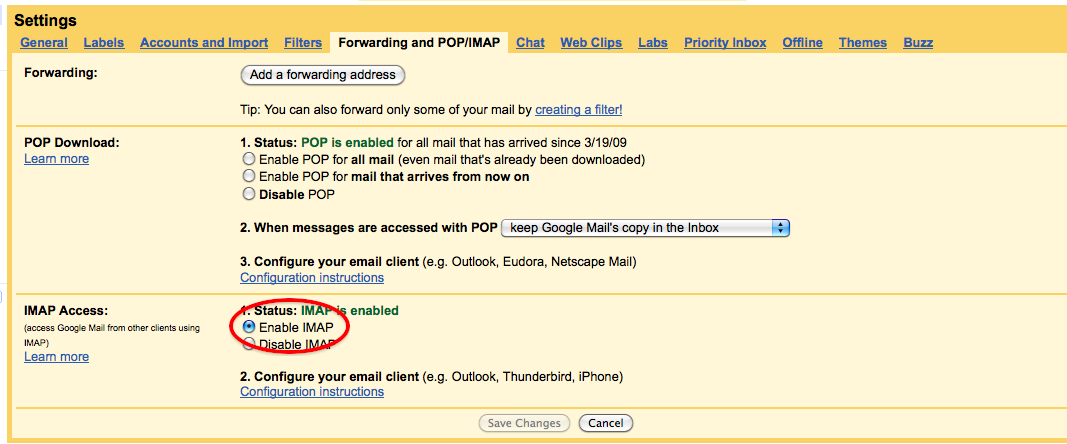
\includegraphics{gmail_imap.png}
\caption{Gmail enable IMAP}
\end{figure}

\subsection{Configuring Thunderbird to use SSL/TLS}

When you start up Thunderbird for the first time, you will enter a
step-by-step configuration procedure for setting up your first account.
(You can invoke the account setup interface any time by selecting
\textbf{File \textbar{} New \textbar{} Mail Account}). On the first
screen, you will be asked for your name, your email-address and your
password. The value you enter for your name does not have to be your
real name. It will be shown to the recipient of your messages. Enter the
information and click \textbf{Continue}.

\begin{figure}[htbp]
\centering
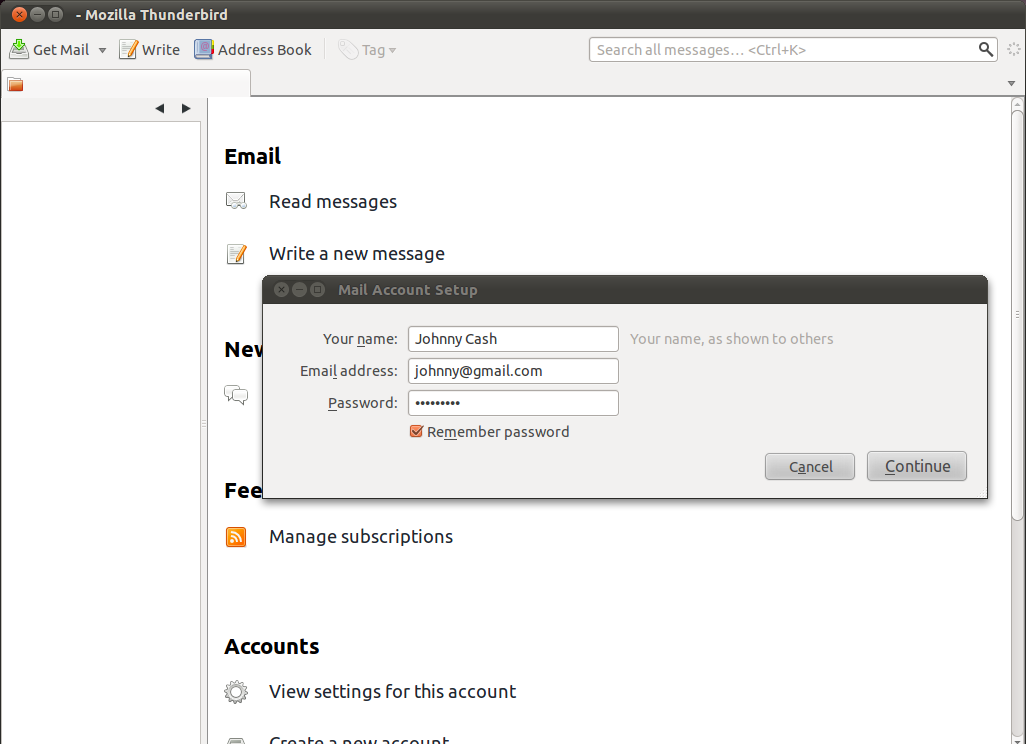
\includegraphics{thunderbird_conf_1.png}
\caption{Thunderbird Configure}
\end{figure}

On the next screen, Thunderbird will attempt to determine the server
names based on your email address. This may take some time, and will
only work if Thunderbird knows the settings for the mail servers for
your email provider. In either case you will be presented with a window
where you can modify the settings. In the example below, Thunderbird has
detected the settings automatically. You can see the protocol at the
right side of the server names. This should be either \textbf{SSL/TLS}
or \textbf{STARTTLS}. \emph{Otherwise your connection is insecure and
you should attempt manual setup.}

\begin{figure}[htbp]
\centering
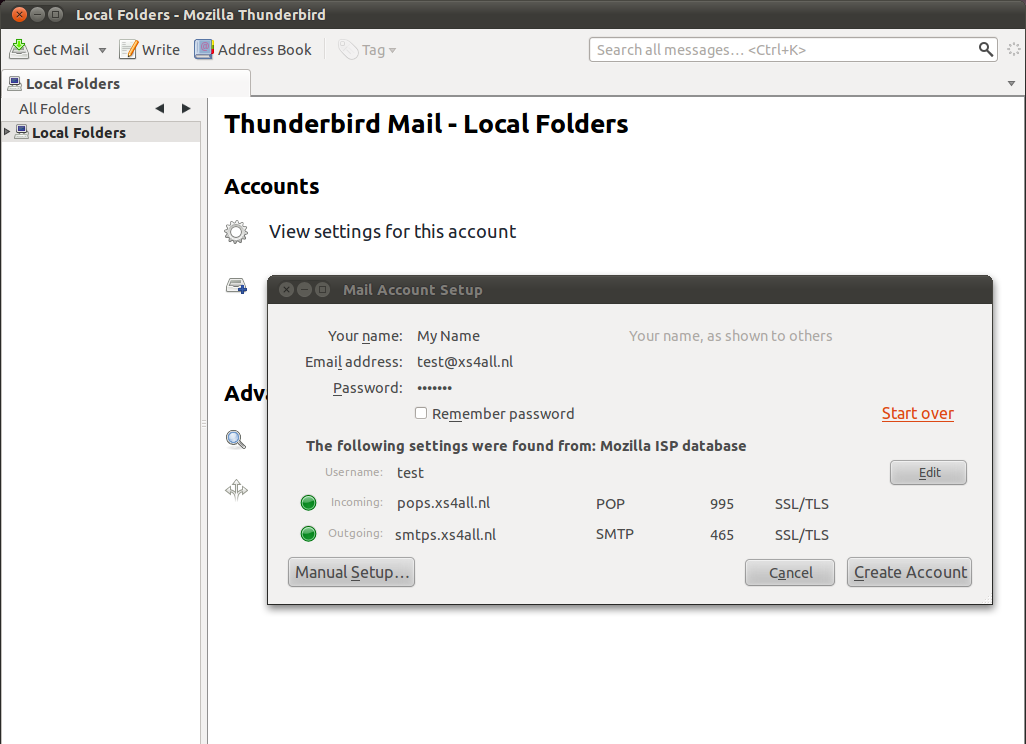
\includegraphics{thunderbird_conf_2.png}
\caption{Thunderbird Install}
\end{figure}

When you are finished, click \textbf{Create account}. If Thunderbird
could not determine your server settings, click on \textbf{Manual setup}
to configure the server names yourself.

\subsection{Manual setup}

Use the Account Settings interface to manually configure accounts in
Thunderbird. The Account Settings dialog will automatically open if you
select \textbf{Manual setup} in the configuration wizard. In this case
we are only interested in the incoming and outgoing mail server names,
and the protocol we use to connect with them. As you can see in the
examples below, we enter the Gmail server names and we force them to use
\textbf{TLS/SSL}, a secure method to connect to the servers.

\begin{figure}[htbp]
\centering
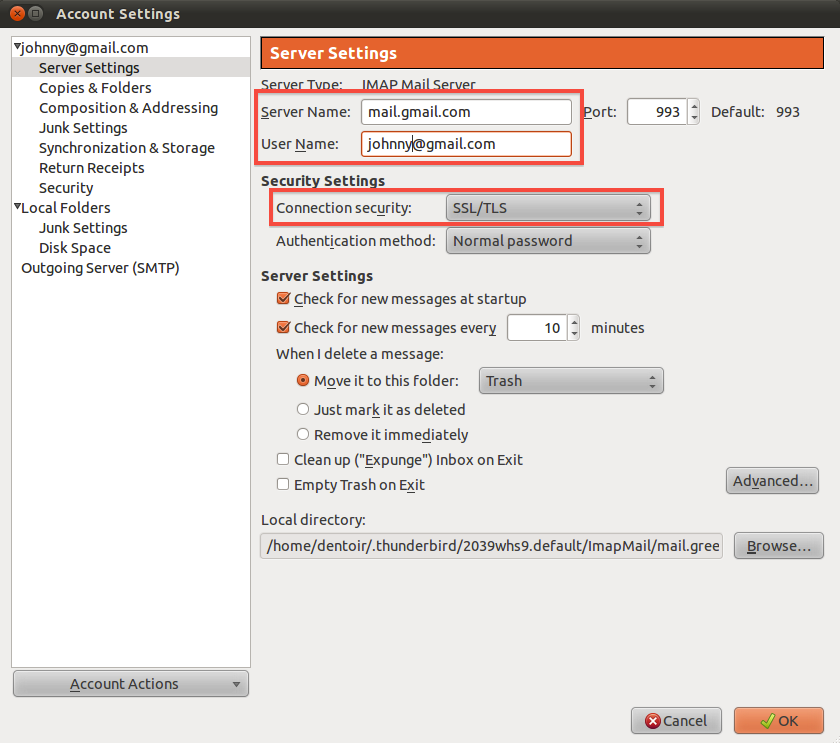
\includegraphics{thunderbird_conf_3.png}
\caption{Thunderbird Install}
\end{figure}

Under `Server Settings', we will find only the incoming (\textbf{IMAP})
server and its settings for that specific account.

\begin{figure}[htbp]
\centering
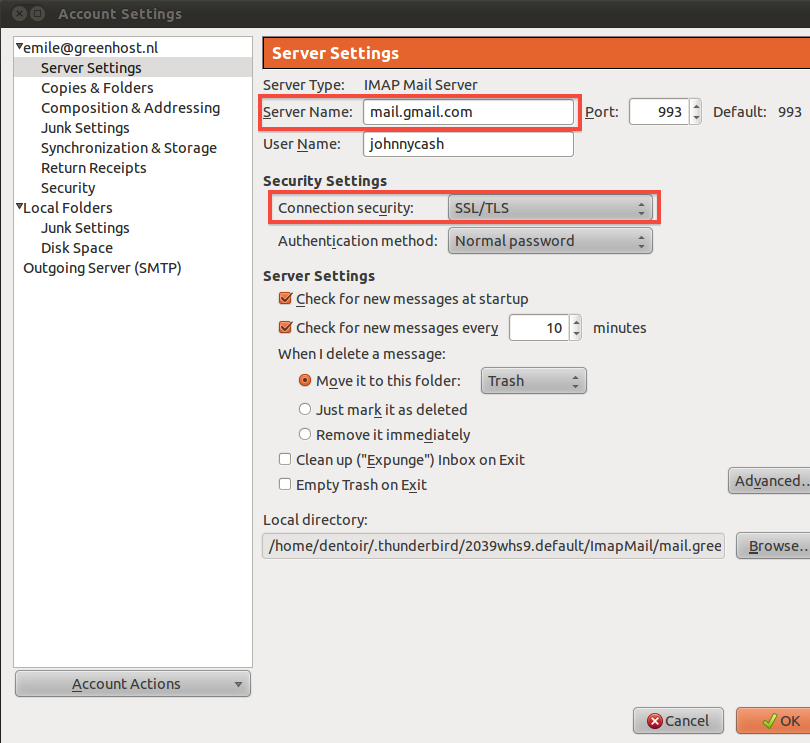
\includegraphics{thunderbird_conf_4.png}
\caption{Thunderbird Install}
\end{figure}

After \textbf{Server Name} enter the name of the IMAP server, in this
case \verb!mail.gmail.com!.

\emph{As you can see we have selected \textbf{`SSL/TLS'} under the
connection security setting. This enforces encryption.} Do not be scared
by the authentication method \textbf{Normal password}. The password will
be automatically encrypted due to our secured connections to the server.

Finally, configure the outgoing server for the account. Click on
\textbf{Outgoing Server (SMTP)} in the left panel.

\begin{figure}[htbp]
\centering
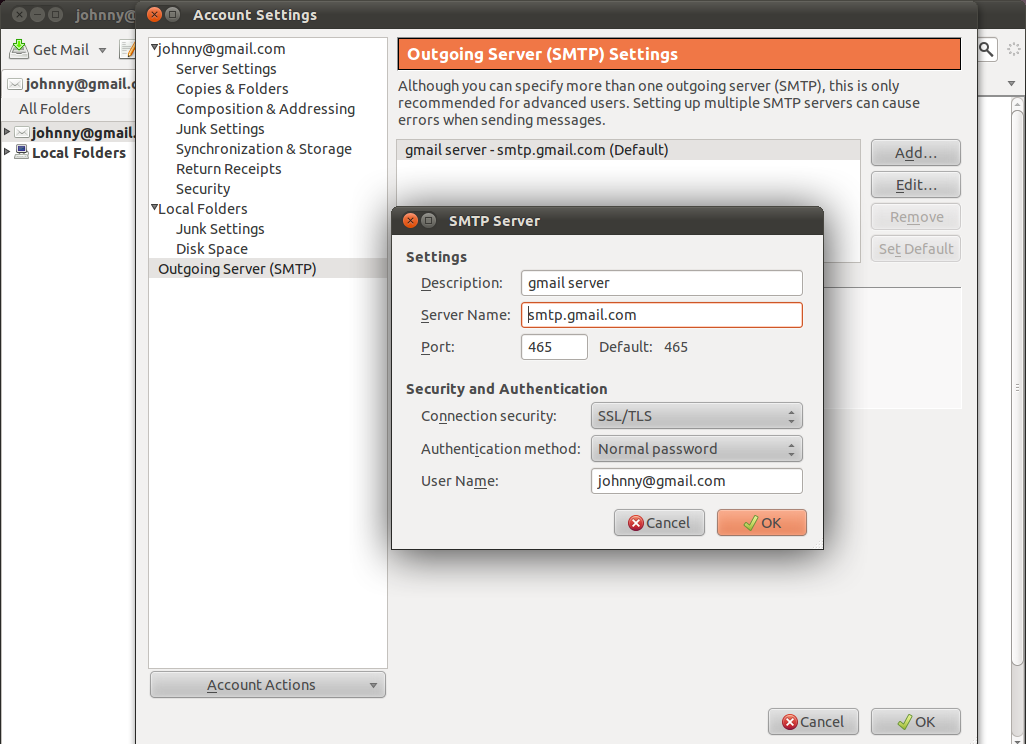
\includegraphics{thunderbird_conf_5.png}
\caption{Thunderbird Install}
\end{figure}

Again, we have selected \textbf{SSL/TLS} under \textbf{Connection
security}. The port will default to 465 and this should generally not
have to be changed.

\subsection{Finishing the setup, different encryption methods}

Test your Thunderbird setup by trying to send and receive mails. Some
email hosting providers may not support the SSL/TLS protocol, which is
the preferred choice. You will get an error message saying the
authentication protocol is not supported by the server. You may then
switch to using STARTTLS instead. In the above two screens, select
`STARTTLS' under `Connection security'. If this method also fails,
contact your email hosting provider and ask them if they provide another
way to securely connect to their servers. If they do not allow you to
securely connect to their servers, then you should complain and
seriously consider switching to a different provider.

\subsection{Returning to the configuration screens}

At any time you can reconfigure your email accounts by going to the
Thunderbird menu bar and clicking \textbf{Edit \textbar{} Account
Settings} (Linux), \textbf{Tools \textbar{} Account Settings} (Windows
and Mac OS X).
